\chapter{An\'alisis temporal y costes de desarrollo}\label{anatemporal}
\section{An\'alisis temporal}
\subsection{Iteraciones}

Dividiremos el trabajo en varias iteraciones, de forma que el proyecto se quede lo más planificado posible para que, a la hora de trabajar, solo haya que seguir las iteraciones:\\

\textbf{Iteración 1}

En esta iteración buscamos dejar empezado tanto el proyecto como la documentación, creando una base sobre la que trabajar más adelante. Además dejamos preparadas las herramientas a utilizar, tanto de trabajo (Microsoft Visual Studio Code, XAMPP), como de redacción (TeXStudio, Google Docs), almacenamiento en la nube (GitHub, Google Drive) y gestión del tiempo (Toggl). Realizamos el primer capítulo de la documentación y diseñamos los mockups.\\

\textbf{Iteración 2}

Planificamos el proyecto de forma que se quede dividido para las siguientes iteraciones y continuamos con la documentación. Redactamos los apartados que podemos (ya que algunos de ellos requieren que se haya avanzado más) de los capítulos 2, 3, 4 y 5. Además se realiza un curso de Angular \citep{cursoangular} para prepararnos para la siguiente iteración.\\

\textbf{Iteración 3}

Esta iteración está pensada como introducción a Angular. Se planea tener lista la página de inicio, el registro de usuario y login, el acceso a perfil y su respectiva información sobre el usuario, así como las diversas acciones que puede realizar desde el mismo (a excepción del álbum de fotos). Se busca establecer la estructura de la base de datos, realizar la vista (final a ser posible) de las páginas mencionadas así como los elementos back-end necesarios para permitir a los usuarios registrarse en la plataforma, loguearse y acceder a su perfil. Además se realizarán las pruebas respectivas.\\

Tras haber realizado la iteración, se descubrió que había cierta diferencia entre lo que pensábamos que sería el perfil y lo que ha acabado siendo (Más información en el capítulo 6).\\

\clearpage

\textbf{Iteración 4}

Se busca implementar la API y los elementos relacionados con esta. Habría que hacer un repaso de lo hecho en la iteración anterior para aplicar las imágenes y valores que se necesiten de la API. Además se planea realizar los distintos catálogos (a excepción del de sueños y canciones) así como el listado de criaturas en tiempo real. Se realizarán las pruebas respectivas.\\

\textbf{Iteración 5}

En esta iteración nos queremos centrar en la implementación de las funciones de calculadora de nabos, calendario de eventos, álbum de fotos, catálogo de sueño, catálogo de canciones y vestuario, así como las pruebas respectivas.\\

Una vez realizada la iteración, tuvimos que afrontar algunas decisiones que han tenido efecto en lo que finalmente se ha acabado desarrollando (Más información en el capítulo 6).\\

\textbf{Iteración 6}

En la última iteración queremos terminar la redacción de la documentación y revisarla de forma que se quede lista para la entrega, arreglar los posibles fallos menores que queden del proyecto, comprobar que la aplicación está terminada y realizar el despliegue.\\

\subsection{Estimación vs Realidad}

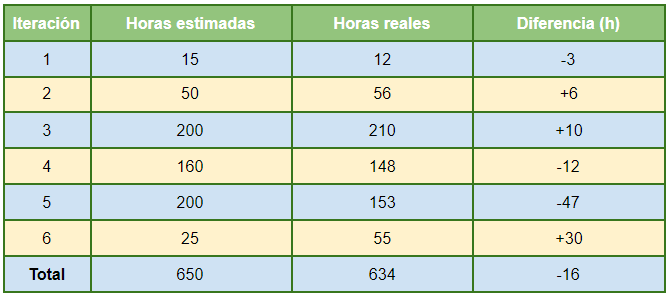
\includegraphics[width=\textwidth]{img/cap4/analisistiempo.png}\\

Al haber eliminado diseños y probador (ver capítulo 6), se han reducido en parte las horas reales en el sprint 5. Sin embargo, debido a que hemos acabado realizando los tests en el sprint 6, así como a los distintos fallos de despliegue a los que nos hemos enfrentado, hemos tenido que dedicarle más tiempo del que pensábamos a dicho sprint, por lo que hemos contado con tiempo de margen y como se puede observar, no ha supuesto un problema respecto a la planificación.

\clearpage

\section{Costes de desarrollo}
	
\subsection{Costes Directos}	

\textbf{Personal}

Dado que aunque sepamos algo de PHP gracias a algunas asignaturas cursadas anteriormente, no tenemos ninguna experiencia con Angular, calcularemos nuestros sueldos clasificándonos como programadores junior. Dicho conjunto cobra una media de 19.000€ al año, lo cual sería 1.584€ al mes, que al dividirlos en un horario de trabajo de 40 horas semanales, 160 horas al mes, equivaldría a 10€ la hora.\\

Esto hay que multiplicarlo por dos ya que el equipo del proyecto está formado por dos personas, es decir, dos programadores junior con sus respectivos sueldos, por lo que sería un total de 20€ la hora.\\

\subsection{Costes Indirectos}

Realizaremos el proyecto en Microsoft Visual Studio Code, un entorno de desarrollo gratuito, en una base de TypeScript con Angular usando el back-end en PHP a modo de API encargado de realizar las peticiones a una base de datos de MariaDatabase (MySQL), cuyas licencias son gratuitas.\\

Para el almacenamiento de datos en la nube usaremos GitHub y Google Drive, los cuales disponen de licencia gratuita con aspectos limitados.\\

Para la redacción utilizaremos tanto Google Docs como TeXStudio, ambos con licencia gratuita.\\

Para la gestión de tiempo y comunicación usaremos Toggl y WhatsApp respectivamente, las cuales también disponen de licencia gratuita (con limitaciones en el caso de Toggl).\\

Los únicos costes indirectos que podríamos encontrar sería la electricidad y la conexión a Internet, lo cual supone de media 35€ por persona, 70€ en total al mes.\\

\subsection{Amortizaciones}

Para realizar el proyecto hemos usado los siguientes equipos:\\

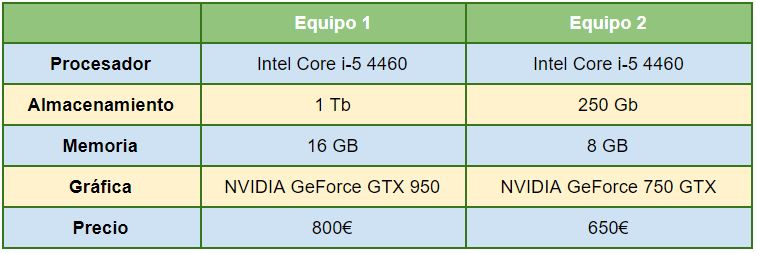
\includegraphics[width=\textwidth]{img/cap4/equipos.jpg}

\bigskip

Además de esto para comunicarnos hemos usado nuestros teléfonos móviles, por eso hemos decidido añadirlo al documento:\\

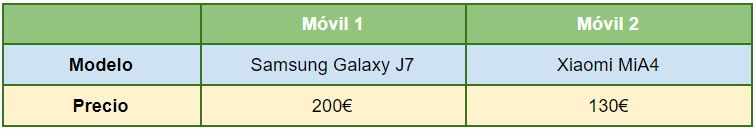
\includegraphics[width=\textwidth]{img/cap4/moviles.jpg}


\subsection{Total}	

Finalmente, sumaremos todos los cálculos anteriores para dar una cifra al precio total:\\

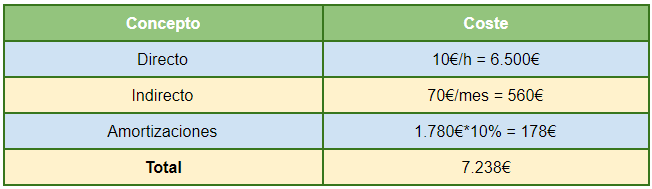
\includegraphics[width=\textwidth]{img/cap4/total.png}



	

	